\label{Konzept}
\chapter{Konzept}

Zum Beispiel:  
- Blockbild der Architektur Ihrer Anwendung  
- Pseudocode für Algorithmen  
- mathematische Formeln  
- evtl. Diagramme auf hohem Abstraktionsniveau.  

\section{Grundkonzept}

 	Das zentrale Element der Applikation bildet der Telegram-Bot selbst. Er wird von einem Benutzer angesprochen und reagiert auf seine Eingabe. So können verschieden Funktionen ausgelöst werden. Bspw. werden Antworten zurückgegeben, Informationen gespeichert oder es wird ein Vorschlag gemacht und an den Nutzer zurückgegeben. Der Bot soll mit mehreren Benutzern gleichzeitig sprechen können. Das wird ermöglicht, weil alle Reaktionen des Bots mit der Kennung des jeweiligen Nutzers verknüpft sind. So spricht der Bot den Nutzer mit Namen an oder kann sich daran erinnnern, welche Fragen schon beantwortet wurden und welche nicht.	 


 \begin{figure} %[hbtp]
	\centering
	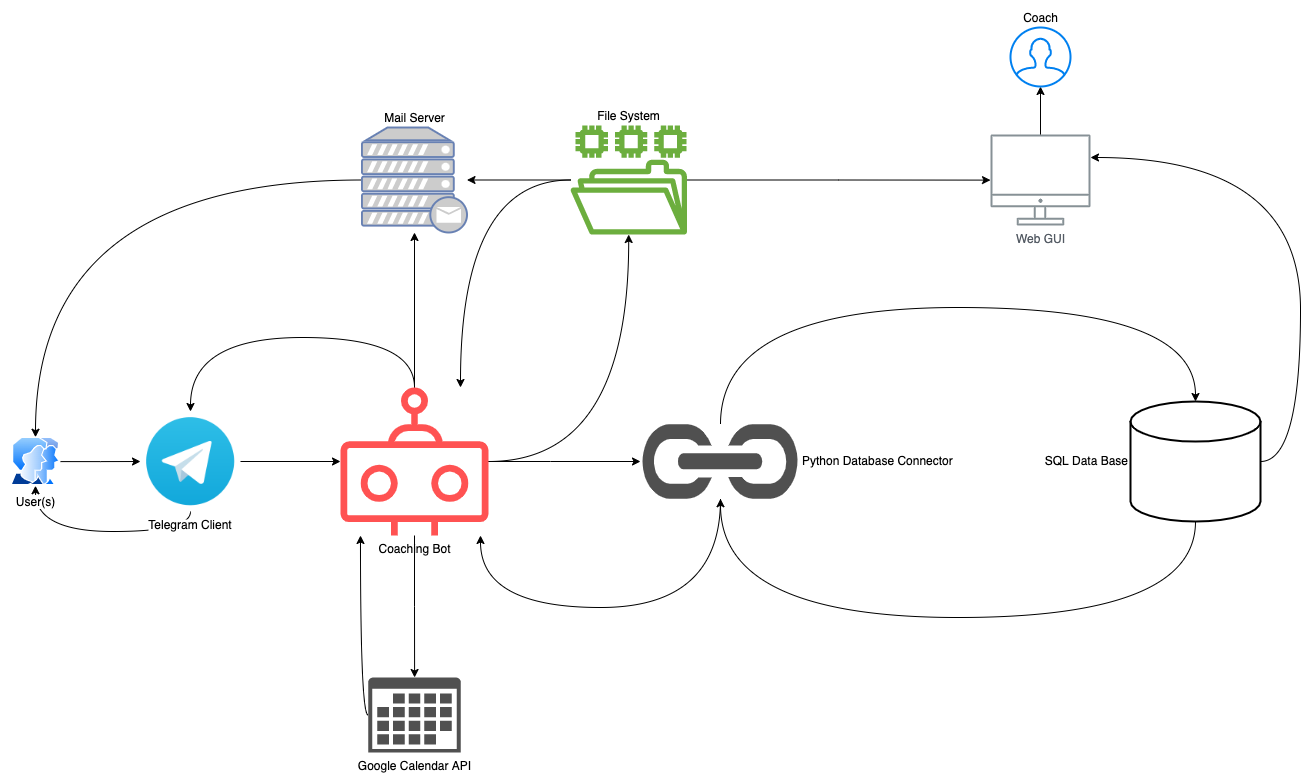
\includegraphics[width=1.0\textwidth]{images/220213_PA28464_Architecture.png}
	\caption{Abstrakte Architektur für das Projekt "Der Coaching Bot"}
	\label{architecture}
\end{figure}


\begin{figure} %[hbtp]
	\centering
	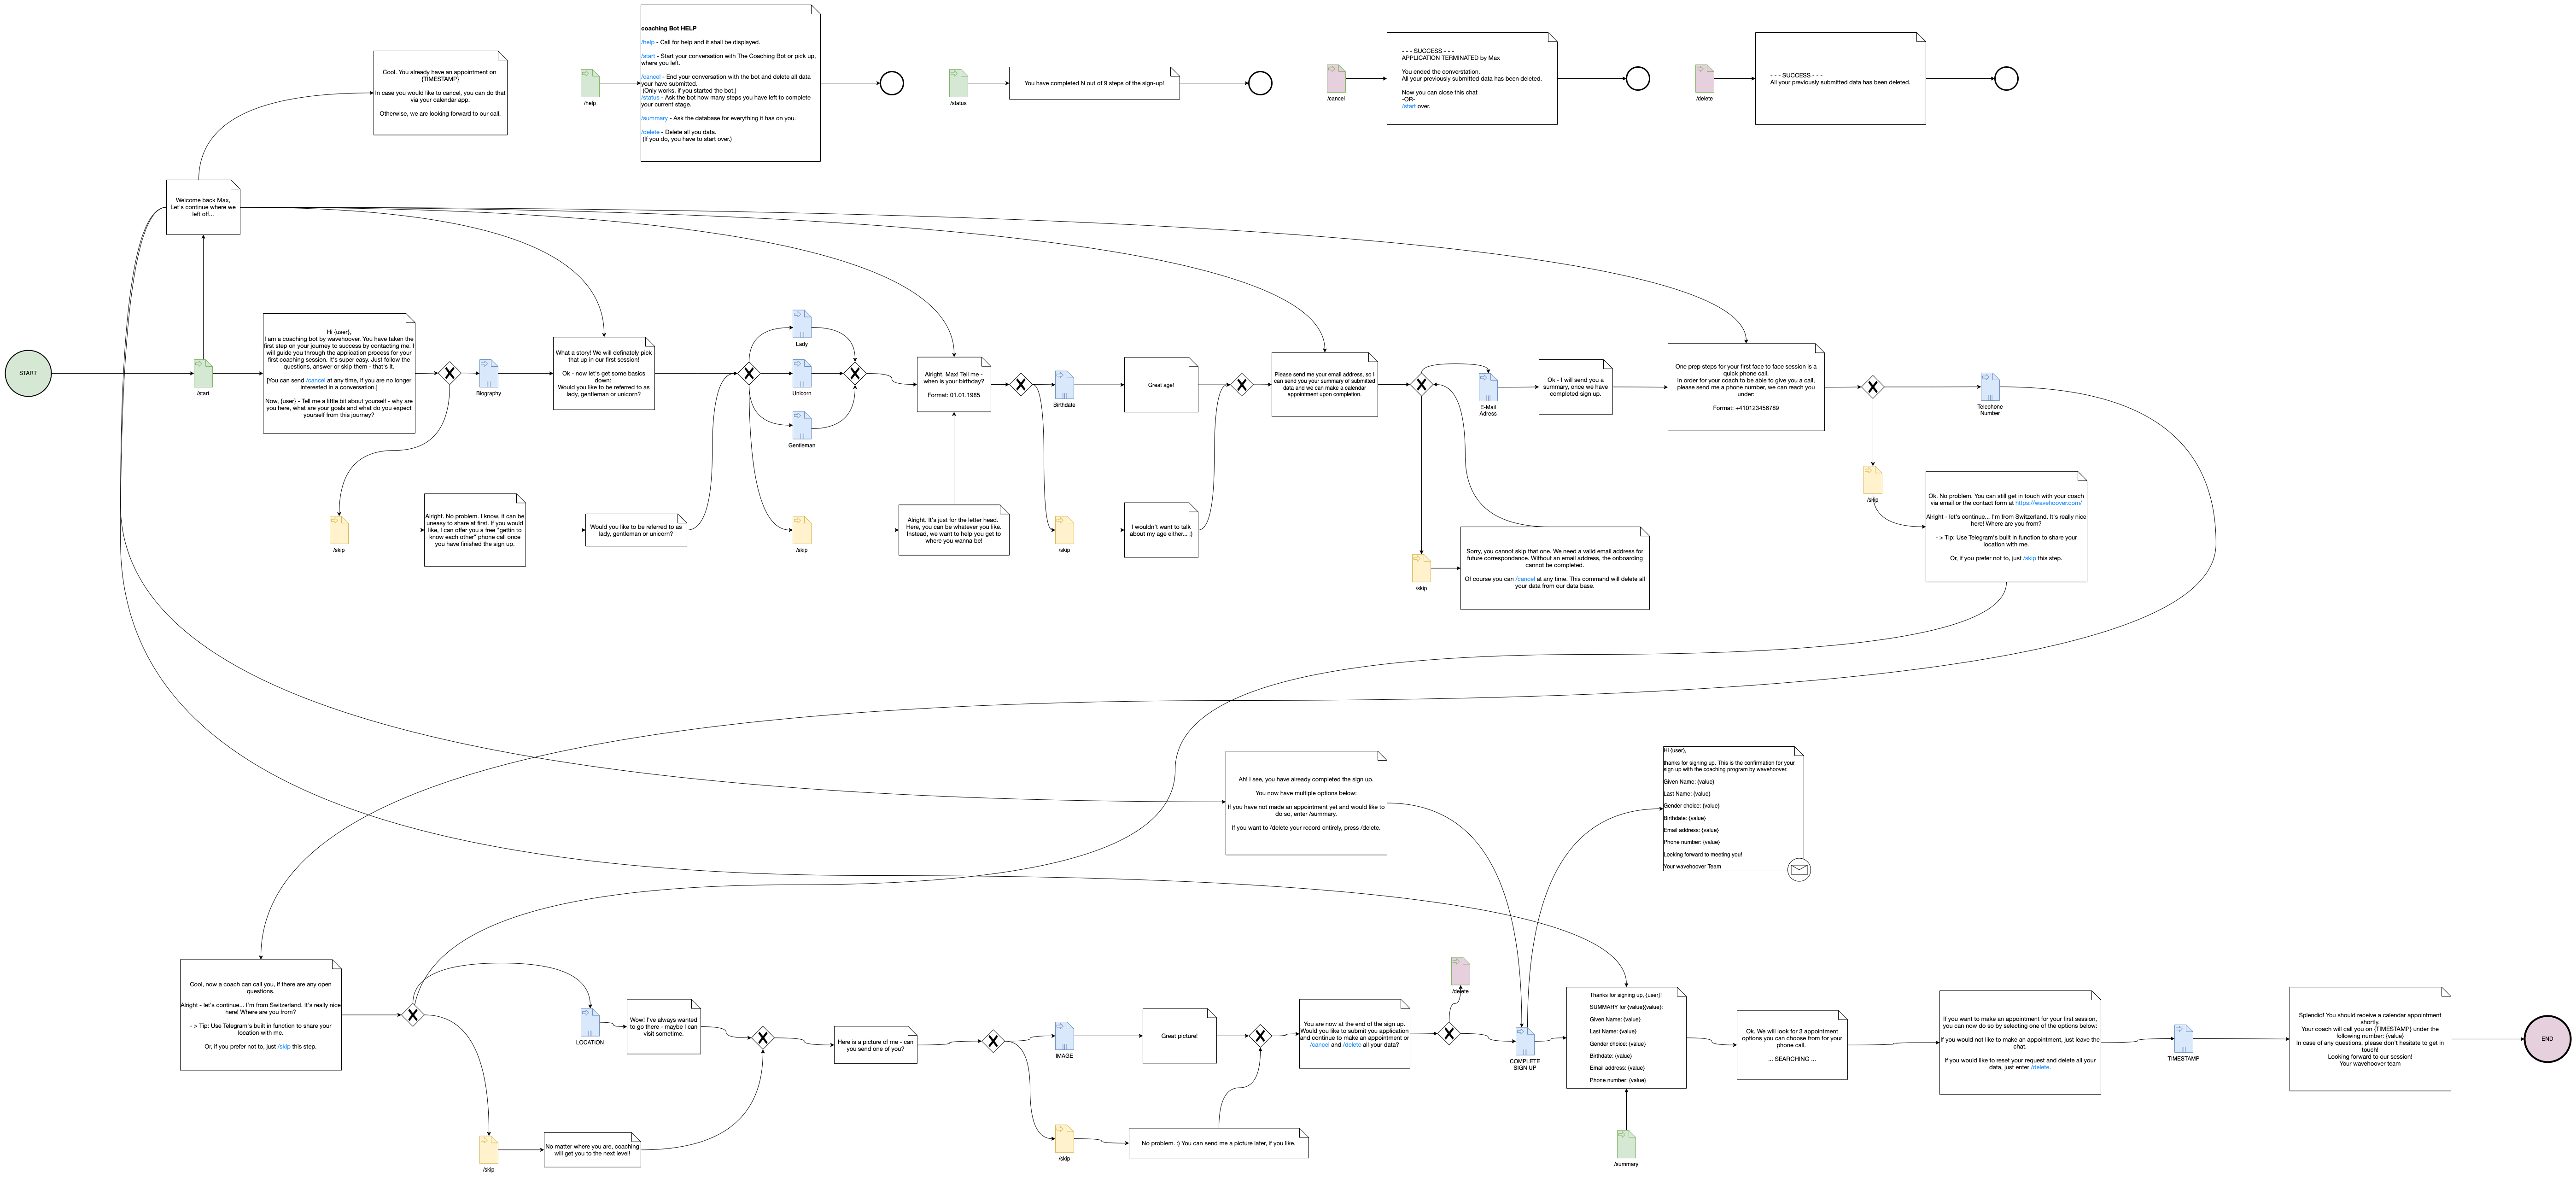
\includegraphics[width=1.0\textwidth]{images/220213_PA28464_Conversation_Flow.png}
	\caption{Konversationsfluss des Bots}
	\label{conversationFlow}
\end{figure}

